\documentclass[tikz,border=9pt]{standalone}
\usepackage{amsmath}
\usetikzlibrary{arrows.meta,angles,quotes,calc}
\definecolor{ink}{HTML}{21352F}
\definecolor{teal}{HTML}{087F7B}
\definecolor{blue}{HTML}{4B77A8}
\definecolor{gold}{HTML}{C58B2A}
\definecolor{rose}{HTML}{B65A62}
\begin{document}
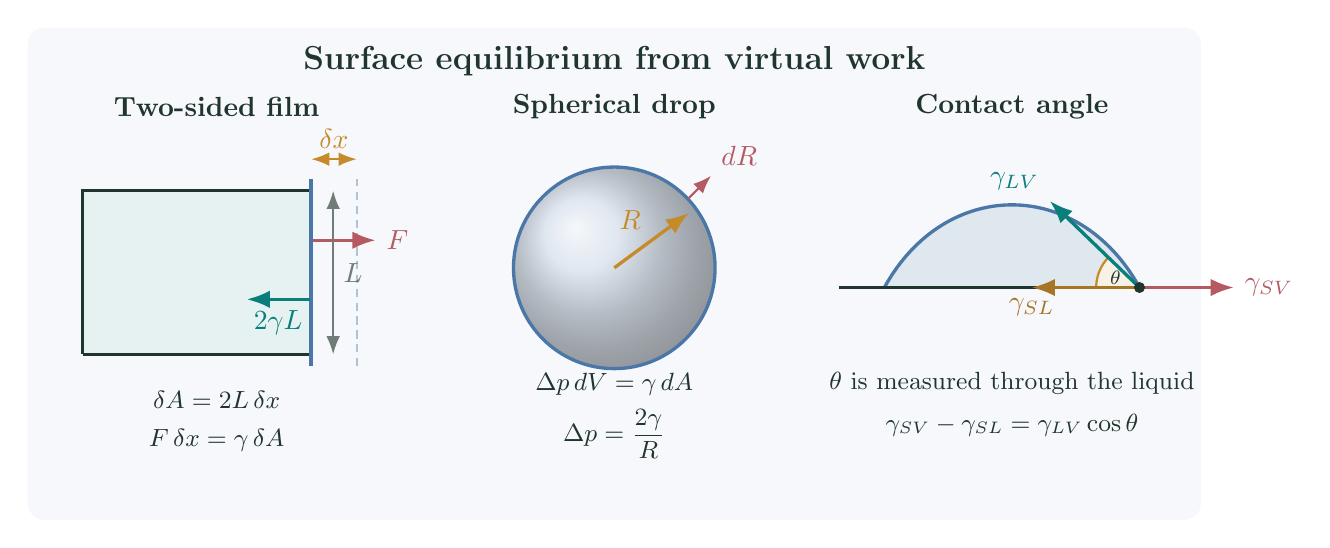
\begin{tikzpicture}[font=\sffamily,text=ink,>=Latex]
  \fill[blue!5,rounded corners=6pt] (-7.45,-3.05) rectangle (7.45,3.2);
  \node[font=\bfseries\large] at (0,2.78)
    {Surface equilibrium from virtual work};

  % Soap-film frame
  \begin{scope}[shift={(-5.05,-.05)}]
    \node[font=\bfseries] at (0,2.25) {Two-sided film};
    \fill[teal!10] (-1.70,-.90) rectangle (1.20,1.18);
    \draw[ink,very thick] (-1.70,-.90)--(-1.70,1.18)--(1.20,1.18);
    \draw[ink,very thick] (-1.70,-.90)--(1.20,-.90);
    \draw[blue,ultra thick] (1.20,-1.05)--(1.20,1.33);
    \draw[densely dashed,blue!45,thick] (1.78,-1.05)--(1.78,1.33);
    \draw[->,rose,very thick] (1.22,.55)--(2.02,.55)
      node[right] {$F$};
    \draw[->,teal,very thick] (1.18,-.20)--(.38,-.20)
      node[midway,below] {$2\gamma L$};
    \draw[<->,gold,thick] (1.20,1.58)--(1.78,1.58)
      node[midway,above] {$\delta x$};
    \draw[<->,ink!65,thick] (1.48,-.90)--(1.48,1.18)
      node[midway,right] {$L$};
    \node[align=center,font=\small] at (0,-1.75)
      {$\delta A=2L\,\delta x$\\[3pt]
       $F\,\delta x=\gamma\,\delta A$};
  \end{scope}

  % Spherical drop
  \begin{scope}[shift={(0,-.05)}]
    \node[font=\bfseries] at (0,2.25) {Spherical drop};
    \shade[ball color=blue!35,opacity=.58] (0,.20) circle (1.28);
    \draw[blue,very thick] (0,.20) circle (1.28);
    \draw[->,gold,very thick] (0,.20)--(.95,.90)
      node[midway,above left] {$R$};
    \draw[->,rose,thick] (.94,1.08)--(1.23,1.37)
      node[above right] {$dR$};
    \node[font=\small,align=center] at (0,-1.68)
      {$\Delta p\,dV=\gamma\,dA$\\[4pt]
       $\displaystyle \Delta p=\frac{2\gamma}{R}$};
  \end{scope}

  % Contact angle on a sessile drop
  \begin{scope}[shift={(5.05,-.10)}]
    \node[font=\bfseries] at (0,2.30) {Contact angle};
    \fill[blue!18]
      (-1.62,0) .. controls (-.85,1.40) and (.85,1.40) .. (1.62,0)
      --cycle;
    \draw[blue,very thick]
      (-1.62,0) .. controls (-.85,1.40) and (.85,1.40) .. (1.62,0);
    \draw[ink,very thick] (-2.20,0)--(2.20,0);
    \coordinate (O) at (1.62,0);
    \coordinate (A) at (.78,.82);
    \coordinate (B) at (.62,0);
    \draw pic[draw=gold,thick,fill=gold!12,angle radius=.55cm,
      "$\theta$" {font=\scriptsize}]
      {angle=A--O--B};
    \draw[->,teal,very thick] (O)--(.48,1.10)
      node[above left] {$\gamma_{LV}$};
    \draw[->,rose,very thick] (O)--(2.82,0)
      node[right] {$\gamma_{SV}$};
    \draw[->,gold!85!black,very thick] (O)--(.25,0)
      node[below] {$\gamma_{SL}$};
    \fill[ink] (O) circle (2pt);
    \node[align=center,font=\small] at (0,-1.48)
      {$\theta$ is measured through the liquid\\[4pt]
       $\gamma_{SV}-\gamma_{SL}=\gamma_{LV}\cos\theta$};
  \end{scope}
\end{tikzpicture}
\end{document}
